\documentclass[usenatbib,a4paper,times]{mnras}

\usepackage{aas_macros}
\usepackage{amsmath}
\usepackage{amssymb}
\usepackage{bm}
\usepackage{breakurl}
\usepackage{graphicx}
\usepackage{natbib}
\usepackage{times}
\usepackage{textcomp}
\usepackage{url}

\newcommand{\st}{\mathrm{St}}
\renewcommand{\sun}{\mathrm{M}_{\odot}}
\renewcommand{\earth}{\mathrm{M}_{\oplus}}
\newcommand{\mcfost}{\textsc{mcfost}}
\renewcommand{\phantom}{\textsc{phantom}}

\title[Super-Earths in TW~Hya]{Super-Earths in the TW~Hya disc}

\author[Mentiplay, Price \& Pinte]{\parbox{\textwidth}{Daniel
   Mentiplay$^{1}$\thanks{daniel.mentiplay@monash.edu}, Daniel J. Price$^{1}$
   and Christophe Pinte$^{1,2}$}\\
   $^{1}$Monash Centre for Astrophysics (MoCA) and School of Physics and
   Astronomy, Monash University, Clayton Vic 3800, Australia \\
$^{2}$Univ. Grenoble Alpes, CNRS, IPAG, F-38000 Grenoble, France}

\pagerange{\pageref{firstpage}--\pageref{lastpage}} \pubyear{2018}

\date{}


\begin{document}
\label{firstpage}
\bibliographystyle{mnras}
\maketitle


\begin{abstract}

We test the hypothesis that the dust and scattered light gaps seen in recent
observations of TW~Hya are caused by planet-disc interactions. We perform global
three-dimensional dusty smoothed particle hydrodynamics simulations, comparing
synthetic observations of our models with dust thermal emission, CO emission and
scattered light observations. We find that the dust gaps observed at 24~au and
41~au can be explained by super-Earth to super-Neptune mass planets
($\sim$~8--24~$\earth{}$). A planet of Saturn-mass or higher can explain the
depth and width of the gap seen in scattered light at 94~au. Our model produces
a prominent spiral arm while there are only hints of this in the data. To
avoid runaway growth and migration of the planets, and to produce axisymmetric
rings in mm dust emission, we require a disc mass of $\lesssim 10^{-3}\,\sun{}$
in agreement with CO observations but 10--100 times lower than the estimation
from HD line emission.

\end{abstract}



\begin{keywords}
protoplanetary discs --- planet-disc interactions --- hydrodynamics ---  stars:
individual (TW Hydrae) --- submillimetre: planetary systems --- infrared:
planetary systems %
\end{keywords}










\section{Introduction}

TW~Hya, our nearest gas-rich protoplanetary disc, was recently imaged by ALMA at
$870\,\mu$m \citep{andrews:2016}. These observations of thermal emission from
$\sim$100$\mu$m dust in the midplane show a series of stunning axisymmetric
gaps. At just $60$~pc \citep{gaia-collaboration:2018} TW~Hya presents a unique
opportunity to observe planet formation on our doorstep. Being a member of the
3--20~Myr old \citep{barrado-y-navascues:2006} TW~Hya association means TW~Hya
is older than the typical disc lifetime of $\sim$~3~Myr \citep{haisch:2001}
implying that planet formation should almost be complete.

\citet{van-boekel:2017} observed TW~Hya in polarized scattered light using the
Spectro-Polarimetric High-contrast Exoplanet REsearch (SPHERE) instrument on
the Very Large Telescope. Scattered light observations trace the small grains in
the upper layers of the gas disc. These grains are tightly coupled to the gas
via drag. Of the two main gaps in the sub-mm dust emission (at 24~au and 41~au)
only the inner gap is observed in the scattered light image.

Estimates of the gas mass in TW~Hya vary over several orders of magnitude.
\citet{thi:2010} use radiative transfer modelling of CO emission to infer a gas
mass $(0.5\textendash 5)~\times~10^{-3}~\sun{}$. Whereas \citet{bergin:2013} use
hydrogen deuteride (HD) observations to infer a disc mass $>0.05\,\sun{}$. At
this mass the self-gravity of the disc is significant and gravitational
instability may lead to disc fragmentation \citep{kratter:2016}.

The characteristic timescale for aerodynamic drag to act on dust grains is
determined by the dimensionless stopping time, or Stokes number, $\st{}$
\citep{weidenschilling:1977, takeuchi:2002}. The Stokes number controls the rate
of vertical settling and radial drift. The Stokes number is proportional to the
grain size and inversely proportional to the gas density. Small grains ($\sim$
$\mu$m) experience high drag and have low $\st{}$. Whereas large grains
($\gtrsim$~cm) are largely decoupled from the gas phase and have high $\st{}$.
Grains with $\st{}\sim1$ experience the greatest rate of settling and drift and
lead to the formation of axisymmetric rings \citep{ayliffe:2012, dipierro:2015}.
The different response of small and large grains to gas drag can be used to
infer the mechanism for the origin of the gaps.

To reproduce the axisymmetric gaps observed in recent ALMA observations, various
mechanisms have been proposed, including: planet-disc interactions
\citep{dipierro:2015}, self-induced dust trapping \citep{gonzalez:2017},
vortices \citep{zhu:2014}, condensation fronts \citep{zhang:2015}, non-ideal MHD
effects \citep{bethune:2016} and zonal flows \citep{johansen:2009,flock:2015}.

In this Letter, we explore the hypothesis that the axisymmetric rings and gaps
in the TW~Hya disc are carved by planets. Our approach is similar to
\citet{dipierro:2015} who explored a similar hypothesis for HL~Tau. We aim to
constrain the planet masses required to explain the observational data on TW~Hya
and to motivate follow up observations.










\section{Methods}
\label{sec:methods}

\subsection{Numerical method}

We perform 3D global simulations of a dusty gas disc with embedded protoplanets
using \phantom{}, a smoothed particle hydrodynamics (SPH) code
\citep{price:2017}. Dust interacts with the gas via a drag force. This allows
the dust to settle to the midplane and to migrate radially. The dust also
interacts gravitationally with the central star and embedded planets. We use a
low disc mass, so the disc is not self-gravitating.

We simulate only one dust grain size. We choose 100~$\mu$m grains with
$\st{}\sim 1$ to ensure efficient settling and radial migration of our simulated
grains. In this regime it is appropriate to use the two-fluid method
\citep{laibe:2012a}. We use $10^7$ particles for the gas, and $2.5\times 10^5$
for the dust. We use a greater number of gas particles to prevent dust becoming
trapped under the gas resolution scale \citep{laibe:2012a}. For 100~$\mu$m-sized
grains, the gas mean free path is large compared with the grain size, and so we
assume Epstein drag \citet{epstein:1924}. We assume spherical grains with a
material density of $3\ $g~cm$^{-3}$. We also perform gas-only simulations to
explore the impact of the outer planet.

We use sink particles \citep{bate:1995} to represent the central star and three
embedded protoplanets. The sink particles interact gravitationally with the disc
and with each other. Gravitationally bound dust and gas within the accretion
radius is accreted onto the sink. For computational efficiency, we set the
stellar accretion radius to be the inner edge of the disc.

\begin{figure}
   \begin{center}
      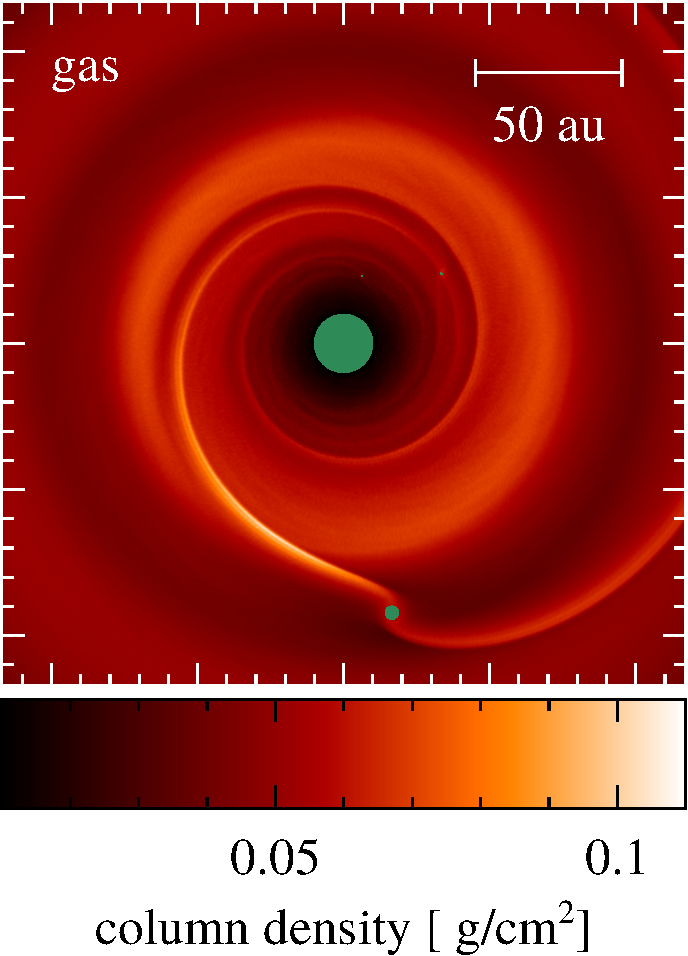
\includegraphics[width=0.496\columnwidth]{figs/gas.pdf}
      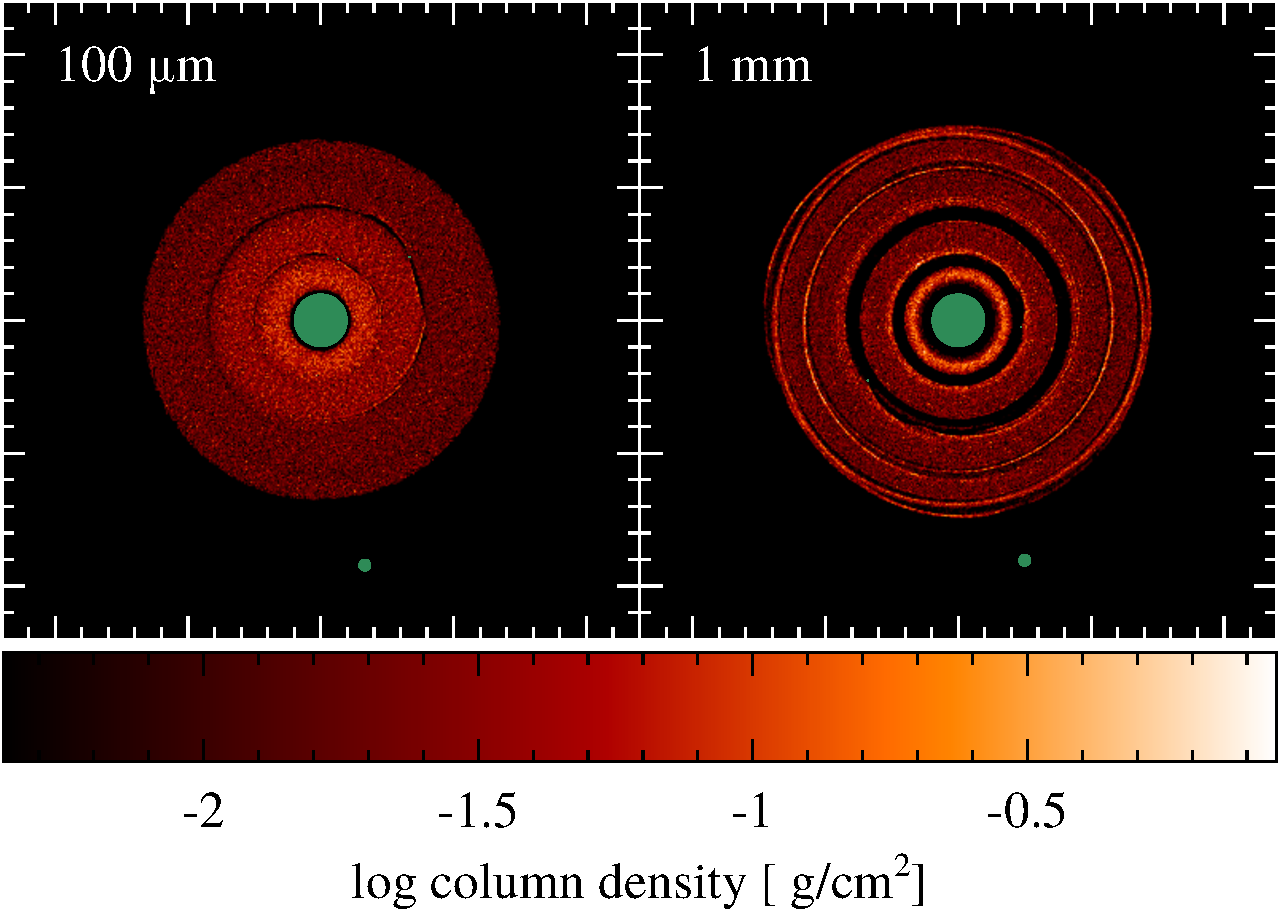
\includegraphics[width=0.496\columnwidth]{figs/dust.pdf}
      \caption{Gas (\textit{left}) and dust (\textit{right}) surface density for
         the model with 8~$\earth{}$ inner planets (24 and 41~au) and
         0.3~$\mathrm{M_J}$ outer planet (94~au) after $14660$~years. The
         green markers are sink particles with radius proportional to accretion
         radius. We do not model the inner ($\lesssim 10$~au) disc. The outer
         edge of the dust disc is $\sim 70$~au.\label{fig:surface-density}}
   \end{center}
\end{figure}

\begin{figure*}
   \begin{center}
      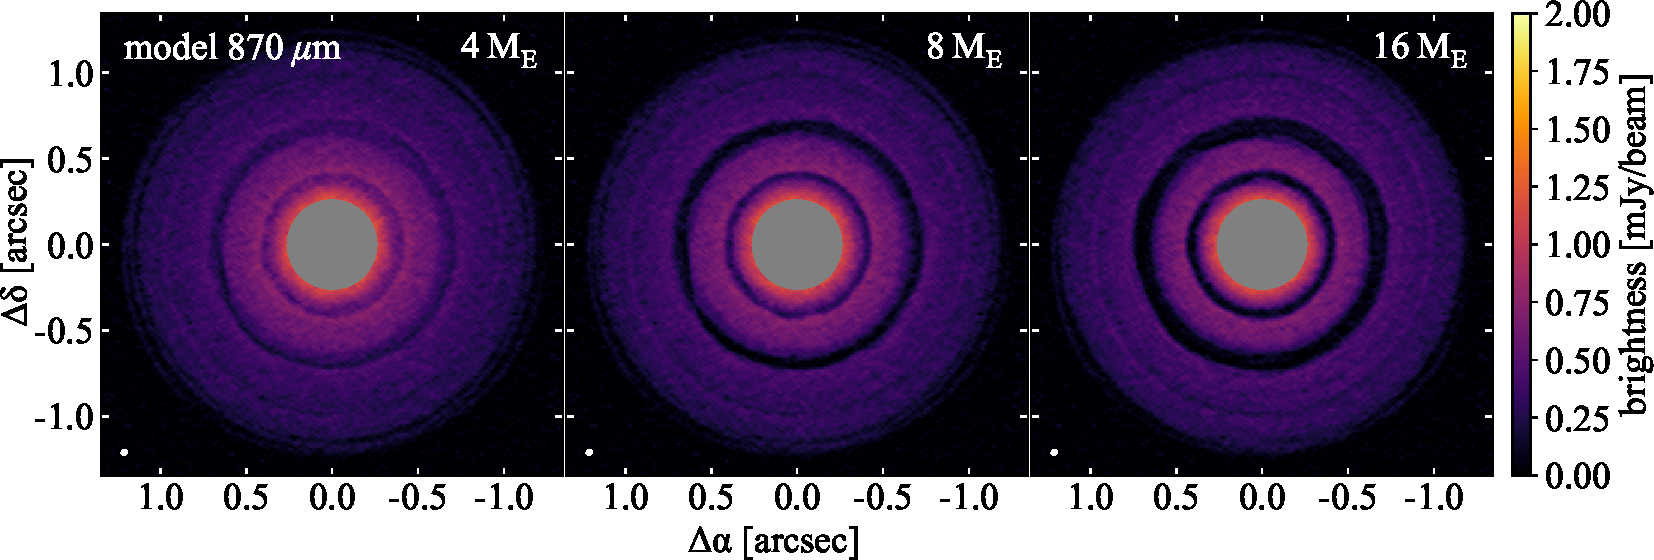
\includegraphics[height=0.200\textwidth]{figs/alma-image.pdf} \quad
      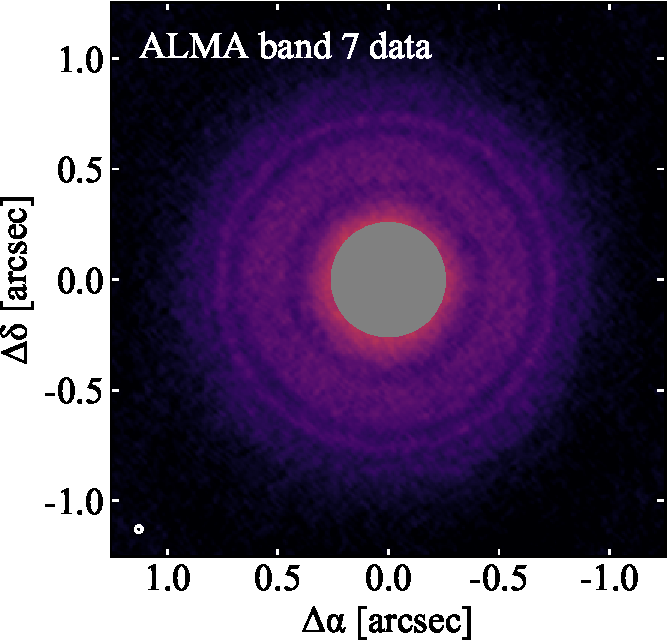
\includegraphics[height=0.200\textwidth]{figs/andrews-2016.pdf}
      \caption{Inner planets (24 and 41~au). Synthetic observations of dust
         thermal emission at $870\,\mu$m, compared with ALMA band 7 observations
         from \citet{andrews:2016}. From left to right: dust+gas models with 4,
         8, 16, 24~$\earth$ inner planets. The beam has FWHM 28$\times$21~mas in
         the model image, compared with 30~mas FWHM ($1.6$~au) circular beam in
         the observations. We obscured the inner $\approx$15~au as we did not
         model that region.\label{fig:alma}}
   \end{center}
\end{figure*}





\subsection{Initial conditions}

We assume a distance of 59.5~au \citep{gaia-collaboration:2016} and a stellar
mass of $0.8\,\sun{}$ \citep{andrews:2012}. Scattered light and CO line
observations show that the gas disc extends out to at least $\sim$200~au
\citep{thi:2010} so we take the outer edge of the gas disc to be 200~au. We set
the inner edge of the disc to be $R_{\mathrm{in}}=10$~au for computational
efficiency. We do not attempt to model the inner disc ($\lesssim$~10~au) in
this study.

We set up a disc consisting of SPH particles following \citet{lodato:2010}. We
assume a gas mass of $7.5\times 10^{-4}\,\sun{}$ (within the annulus from 10~au
to 200~au) which is in the low end of the \citet{thi:2010} range. We set the
initial surface density profile as a smoothed power law: $\Sigma =
\Sigma_{\mathrm{in}} {(R/R_{\mathrm{in}})}^{-p} (1-\sqrt{R_{\mathrm{in}}/R})$,
where we adopt a shallow surface density profile with $p=0.5$. This, with our
gas disc mass, gives a surface density of $\Sigma \approx 0.05-0.08\
$g~cm${}^{-2}$, corresponding to a Stokes number of $\st{}\approx 0.25-0.4$ for
100~$\mu$m grains.

We assume a vertically isothermal equation of state $P={[c_s(R)]}^2\rho$ with $T
= 30\,\mathrm{K} {(R/R_{\mathrm{in}})}^{-0.25}$ where $c_s^2={k_B}T/\mu m_p$.
This is determined by matching the CO snowline (20~K at 19~au) from
\citet{vant-hoff:2017} together with a midplane temperature of 15~K at 60~au
following previous modelling \citep{andrews:2012}. From these we infer a disc
aspect ratio of $H/R = c_s/(\Omega R) = 0.034$ at $R_{\mathrm{in}}$.
\citet{flaherty:2018} provide an upper limit on the turbulent velocity in the
outer disc of $v_{\mathrm{turb}}/c_s\approx 0.04-0.13$. This corresponds to an
$\alpha \sim {(v_{\mathrm{turb}}/c_s)}^2 \lesssim 0.002-0.02$. We choose a disc
viscosity \citep{shakura:1973} at the lower end of this range and set the SPH
artificial viscosity to $\alpha_{\mathrm{AV}} = 0.1$ giving $\alpha \sim 0.001$.

The dust disc is much more compact than the gas disc. Thermal emission from the
dust shows that the sub-mm dust disc extends to $\sim$ 50~au
\citep{andrews:2016}. We set the outer edge of the dust disc to
$R_{\mathrm{out}}=80$~au, just inside the orbital radius of the outer planet.
This is to allow for some radial drift, without having to follow the drift of
dust particles from the gas outer radius. We use the same inner edge as for the
gas disc. Dust disc mass estimates are in the range $(2$--$6)\times
10^{-4}\,\sun{}$ \citep{calvet:2002, thi:2010}. With our gas disc mass this
gives a dust-to-gas ratio of $\approx$~0.25--0.8 which is one to two orders of
magnitude higher than the typical interstellar value. However, TW~Hya is an old
disc within which we can expect significant evolution away from its initial
conditions. We set the dust-to-gas ratio (for 100~$\mu$m grains) to 0.05.





\subsection{Embedded planets}

We assume two super-Earth to super-Neptune mass planets at 24~au and 41~au,
respectively, to reproduce the two main observed gaps in sub-mm emission
\citep{andrews:2016}. We explored masses in the range of 4--24~$\earth{}$ for
these planets. To reproduce the outer gap observed in scattered light
\citep{van-boekel:2017} we placed a more massive planet at 94~au. We explored a
range of masses for the outer planet between 0.1--$2~\mathrm{M_J}$. We set the
planetary accretion radius $R_{\mathrm{acc}}$ to half the Hill radius,
$R_{\mathrm{H}} = a\sqrt[3]{m_{\mathrm{p}}/3M_*}$, where $a$ is the semi-major
axis, and $m_{\mathrm{p}}$ and $M_*$ are the planet mass and stellar mass,
respectively. Accretion proceeds unchecked for particles within 80\% of the
accretion radius.





\subsection{Synthetic observations}

We use the 3D radiative transfer code \mcfost{} \citep{pinte:2006, pinte:2009}
to post-process the \phantom{} output to produce simulated ALMA band 7 images,
CO maps and polarized scattered light images. We use a Voronoi (unstructured)
mesh using Voro++ \citep{rycroft:2009} in which the computational domain is
subdivided into cells generated from the positions of the SPH gas particles. We
assume an inclination of $5^{\circ}$ and position angle $152^{\circ}$
\citep{huang:2018} when making synthetic observations of the disc.

Within each cell we split the distribution of dust grain sizes into 100
logarithmic bins from 0.03~$\mu$m to 1~mm. Grains smaller than 1~$\mu$m are
assumed to trace the gas. Grains larger than 100~$\mu$m are assumed to trace the
dust particles. Grains of intermediate size are interpolated between the gas and
dust. The total dust mass is set to $2.5\times 10^{-4}\,\sun{}$. We use $10^7$
photon packets to determine the temperature structure and $10^7$ photon packets
per wavelength to produce synthetic observations.

We use the Common Astronomy Software Application (CASA) ALMA simulator (version
4.7) to produce synthetic band 7 ALMA images at 870~$\mu$m to compare with
\citet{andrews:2016}. We use a transit duration of 45 minutes, add thermal noise
from the receivers and atmosphere, and set the precipitable water vapour to
$0.5$~mm. To match the beam size of the observations, we choose an ALMA antenna
configuration (cycle 3.8) which gives a beam of FWHM 28$\times$21~mas at
$\mathrm{PA}=-60.3^{\circ}$.

We post-process gas-only \phantom{} simulations in \mcfost{} to produce
polarized scattered light images, and CO emission maps, assuming the dust
follows the gas. In these calculations we assume a dust-to-gas ratio of 0.01.
From 1.6$\,\mu$m (H-band) scattered light maps we calculated the azimuthal
Stokes component $Q_{\phi}$, scaled by $R^2$. We then we add Gaussian noise and
convolve with a Gaussian beam with a FWHM of $48.5$~mas, following the H-band
SPHERE observations in \citet{van-boekel:2017}.

We also produce CO emission maps in the J~=~3~---~2 line. We assume
$T_{\mathrm{gas}} = T_{\mathrm{dust}}$ and that the emission is at LTE, as we
are looking at low-J CO lines. We assume a CO-to-H${}_2$ molecular abundance of
$10^{-4}$. We produce channel maps at 0.1~km/s resolution to then calculate the
$M_0$ moment map. We convolve with a Gaussian beam with FWHM of
139$\times$131~mas with a $\mathrm{PA}=-74.9^{\circ}$ following the ALMA
observations presented by \citet{huang:2018}.

\begin{figure*}
   \begin{center}
      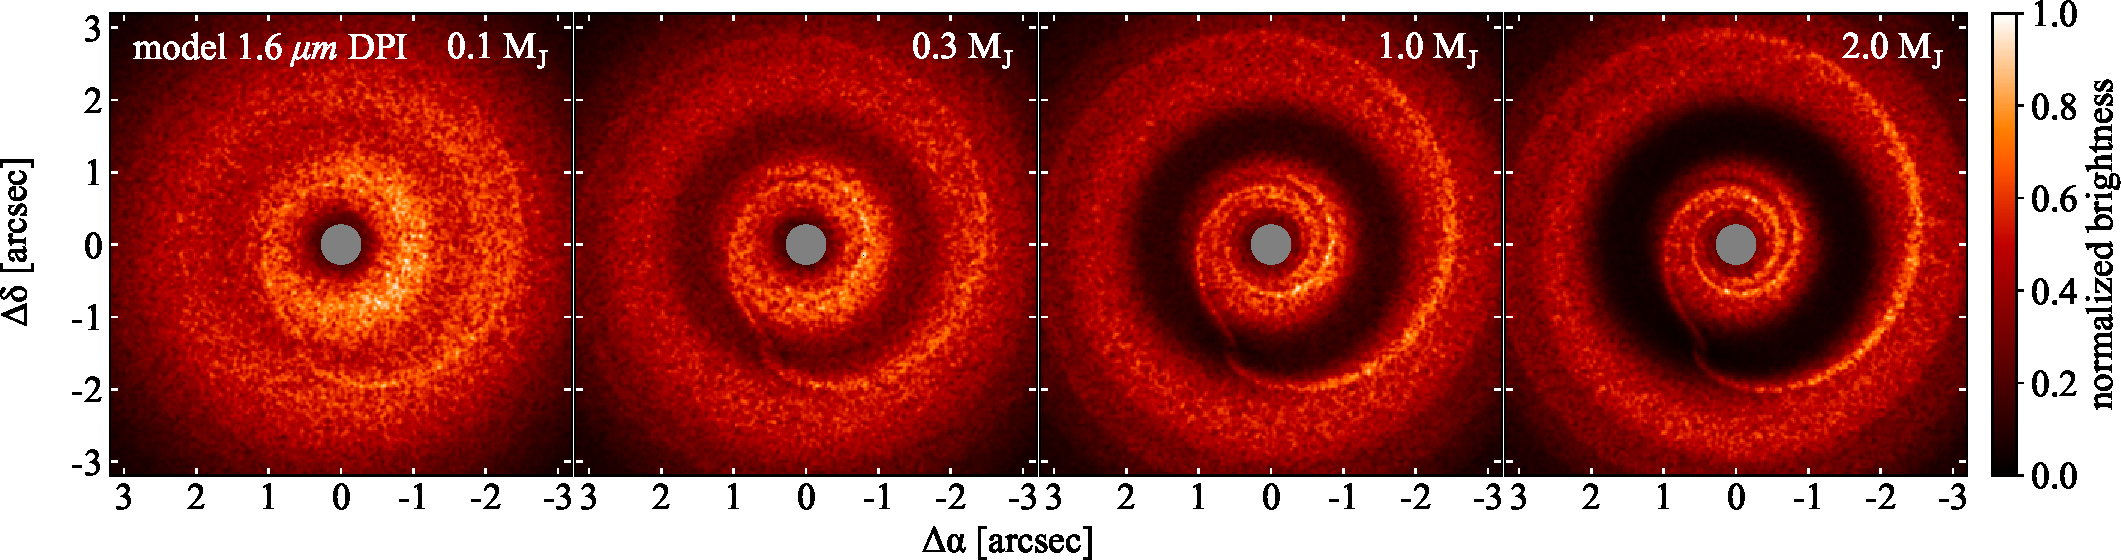
\includegraphics[height=0.206\textwidth]{figs/scattered-image.pdf} \quad
      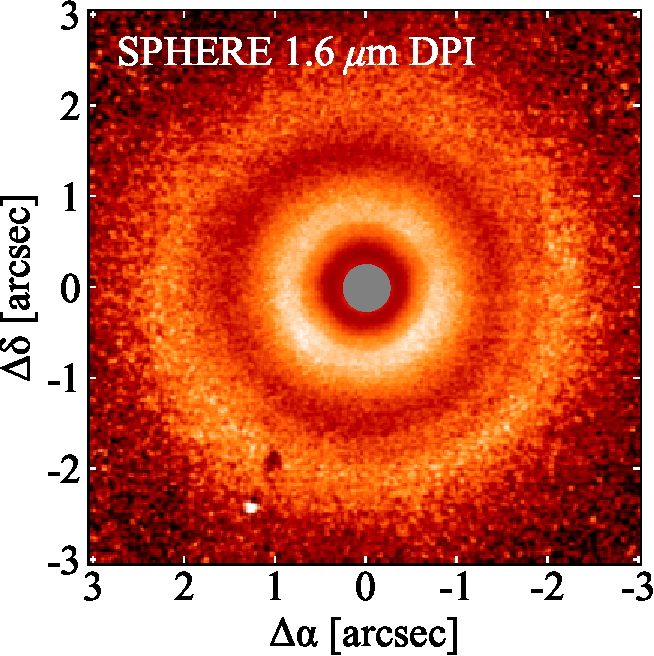
\includegraphics[height=0.206\textwidth]{figs/van-boekel-2017.pdf}
      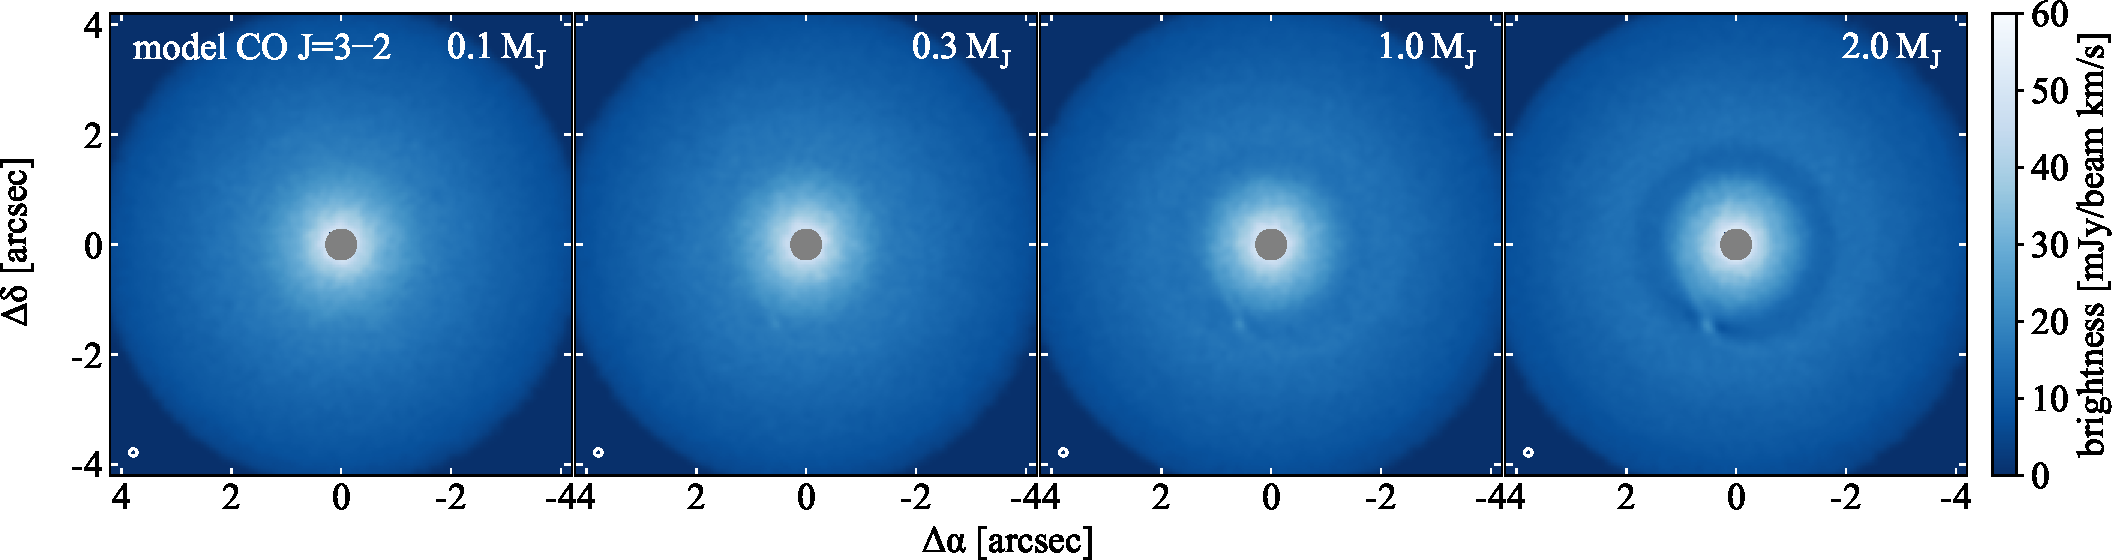
\includegraphics[height=0.206\textwidth]{figs/CO-image.pdf} \quad
      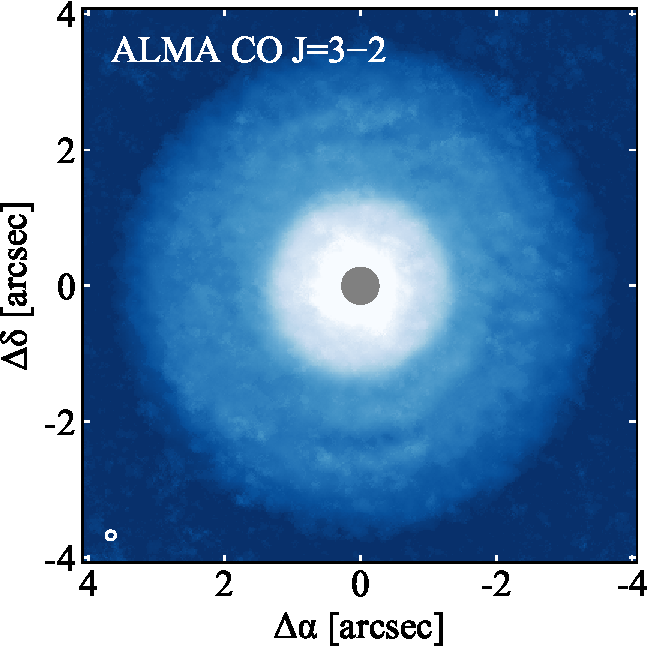
\includegraphics[height=0.206\textwidth]{figs/huang-2018.pdf}
      \caption{Gas-only models with outer planet (94~au) masses 0.1, 0.3, 1, and
         2~$\mathrm{M_J}$ after 45 orbits. \textit{Top}: Comparison of synthetic
         observations of $1.6$~$\mu$m polarized intensity scaled by $R^2$ with
         the SPHERE observation. We convolved with a circular Gaussian beam of
         FWHM $48.5$~mas, and added Gaussian noise. \textit{Bottom}: Comparison
         of synthetic CO J~=~3~---~2 integrated intensity emission maps with the
         ALMA observation. We convolved with a Gaussian beam of
         139$\times$131~mas with a $\mathrm{PA} = -74.9^{\circ}$. The top and
         bottom right panels are reproduced from \citet{van-boekel:2017} and
         \citet{huang:2018}, respectively.\label{fig:scattered-CO}}
   \end{center}
\end{figure*}










\section{Results}
\label{sec:results}

Figure~\ref{fig:surface-density} shows the gas and dust surface density after
14660~years (125, 50, and 16~orbits of the 24, 41, and 94~au planets, resp.) for
the model with 8~$\earth{}$ inner planets (24 and 41~au) and 0.3~$\mathrm{M_J}$
outer planet (94~au). The dust disc extends to $\sim 70$~au (\textit{right} of
Figure~\ref{fig:surface-density}). We note that there was negligible planetary
migration. We observe cleared dust gaps at the locations of the two inner
planets, while the planets are not massive enough to carve gaps in the gas
(Figure~\ref{fig:surface-density}). The Saturn-to-Jupiter-mass outer planet
carves a (partial) gap in the gas, and produces a spiral density wave. The
region interior to 10~au is devoid of dust merely because it is within the
accretion radius of the stellar sink particle.





\subsection{Dust thermal emission}

Figure~\ref{fig:alma} compares our synthetic band 7 ALMA observations of dust
thermal continuum emission for models with 4, 8, 16, and 24~$\earth{}$ inner
planets with the ALMA observations \citep{andrews:2016}. Low mass planets ($<
0.1\,\mathrm{M_J} \approx 32\,\earth{}$) successfully reproduce the width and
axisymmetry of the observed gaps at 24 and 41~au.

Increasing the planet mass increases the gap width, as expected. No gap is
opened by a 4~$\earth{}$ planet at 41~au. The lowest mass planets that can
produce almost axisymmetric gaps for our disc model at both 24 and 41~au is
$\approx\,$8~$\earth{}$. The planet mass with gap width closest in size to the
ALMA gap width of $\approx\,$5~au depends on orbital radius. Our results suggest
that to carve a 5~au gap at 24~au in the 100~$\mu$m dust disc requires a planet
mass of 16--24~$\earth{}$. Similarly, to carve a 5~au gap at 41~au in the
100~$\mu$m dust disc requires a planet mass of 8--16~$\earth{}$. This suggests
that the 24~au planet is more massive than the 41~au. This finding is consistent
with the scattered light observations, which show a low contrast gap at 24~au
but none at 41~au. A planet mass of 16--24~$\earth{}$ for the innermost planet
is also consistent with an upper limit suggested by \citet{nomura:2016}. It is
also consistent with modelling from \citet{van-boekel:2017} following
\citet{duffell:2015}, and with the low-viscosity models of \citet{dong:2017b}.





\subsection{Scattered light and CO emission}

Figure~\ref{fig:scattered-CO} (\textit{top}) compares our synthetic polarized
scattered light H-band observations for gas-only models with outer planet masses
0.1, 0.3, 1, and 2~$\mathrm{M_J}$, with the SPHERE observation from
\citet{van-boekel:2017}. The spiral density wave induced by the outer planet is
visible in all of our synthetic observations. For the 0.3, 1, and
2~$\mathrm{M_J}$ we observe a dip in scattered light at the orbital radius of
the planet.  Figure~\ref{fig:scattered-radial} quantifies this by comparing the
azimuthally-averaged brightness profile for each model. The brightness contrast
between the peak and gap for a Saturn to Jupiter mass (0.3--1~$\mathrm{M_J}$)
planet is consistent with the SPHERE observation. A 0.1~$\mathrm{M_J}$ planet,
by contrast, fails to reproduce the gap.

Figure~\ref{fig:scattered-CO} (\textit{bottom}) compares synthetic
CO~J~=~3~---~2 emission maps for gas-only models with outer planet masses 0.1,
0.3, 1, and 2~$\mathrm{M_J}$, with the ALMA observations \citep{huang:2018}. The
0.3--1~$\mathrm{M_J}$ models, which best fit the scattered light radial profile,
is consistent with CO observations. For a planet larger than 0.3~$\mathrm{M_J}$,
the gas surrounding the planet is visible in the $M_0$ map.  This is because we
have infinite signal-to-noise in our model. The gas surrounding the planet has a
perturbed velocity field and is emitting in a large number of channels. While
the signal in each channel is faint and would not have been detected by ALMA,
when aggregated in the $M_0$ map, it becomes visible.  Higher S/N ALMA
observations might be able to detect such a signal.










\section{Discussion}
\label{sec:discussion}

For computational efficiency we did not model the inner disc (within
$\sim$~10~au). This leads to a hotter temperature at radii $\lesssim 15$~au,
where the stellar radiation directly hits the dust. Thus the dust thermal
emission within the innermost planet orbit is larger than the observation. We
checked that the temperature at the location of the planet is not affected by
this, and the corresponding fluxes are correct.

The overall flux is consistent to within a factor of 2 of the ALMA observation.
However, the contrast in flux between our gaps and rings is greater than the
observed contrast. The emission gaps are only 5--20$\%$ fainter than the rings
in the ALMA observations \citep{andrews:2016}. Whereas the model gaps are
60--80\%. This is likely due to our choice to only simulate one grain size for
the population of large grains. We expect there to be additional flux
contributed from nearby grain sizes that we have not included in our
calculation. These grains will have a different Stokes number than the
100-$\mu$m-grains and will be less effected by the dynamical gap opening of the
planets, thus filling out the flux in the gap. Multigrain dust simulations that
include a range of grain sizes that contribute to the emission wavelength may
alleviate that problem \citep{hutchison:2018}.

Spectral index observations from \citet{huang:2018} suggest that within the gaps
the maximum grain size is at most a few mm, whereas in the bright rings cm
grains are present. In this case, the gas disc mass may be an order of magnitude
higher, such that the mm grains have similar Stokes number to the 100~$\mu$m
grains in our calculations.

There is a tension between the outer planet mass required to reproduce the gap
in scattered light and CO observations, and the mass required to hide a spiral
density wave. The synthetic observation from the $0.3~\mathrm{M_J}$ model (top
of Figure~\ref{fig:scattered-CO}) shows a greater degree of azimuthal asymmetry
than the SPHERE observation. Models with a lower mass planet ($\sim
0.1\,\mathrm{M_J}$) are more azimuthally symmetric. However, at those masses we
fail to reproduce the gap in both scattered light and in CO emission. A mass of
0.3~$\mathrm{M_J} \approx 95$~$\earth{}$ is higher than suggested by previous
authors \citep{dong:2017b, van-boekel:2017}. It is possible that we are
overestimating the planet mass if the gap were accentuated by shadowing from the
inner disc \citep{debes:2013, debes:2017, poteet:2018}.

For our disc model, the stellar accretion rate is $1.5\times
10^{-10}\,\sun{}\,\mathrm{yr}^{-1}$ which is an order of magnitude below the
estimated rate \citep{brickhouse:2012}. The accretion rate is given by $\dot{M}
= 3\pi\Sigma\alpha c_s H$. This suggest two modifications to our model to
increase $\dot{M}$: we could increase the disc mass, and we could increase the
disc viscosity. The are problems with both approaches. Increasing the disc mass
changes the Stokes number of grains. The viscosity is constrained by
observations \citep{flaherty:2018}. An alternative may be that accretion is
driven by winds \citep{simon:2017a} rather than a disc viscosity.

Increasing the stellar accretion rate via either approach increases the
planetary accretion rate. For the $8\,\earth{}$ model the inner planets (24 and
41~au) accrete $\sim\,$1~$\earth{}$ each over the $\approx 15000$~yrs of
simulation time. Extrapolating this rate to over a million years leads to
accretion of $\approx$~50~$\earth{}$, which is uncomfortably high. Increasing
the disc viscosity also requires larger planets to form gaps initially as a
greater gravitational torque is required to overcome the viscous torque from the
gas \citep{dipierro:2016}.

The product of planetary mass and accretion rate $M_p\dot{M_p}$ for the outer
planet (94~au) in the $0.3~\mathrm{M_J}$ model is $2\times 10^{-7}\,
\mathrm{M_J^2/yr}$, which is a factor of 5 greater than the upper limit deduced
from Keck/NIRC2 vortex coronagraph observations \citep{ruane:2017}. Given that
our model constrains the planet mass via the gap depth this suggests that the
accretion rate may be too high in our model. We use a relatively large sink
radius for computational reasons. A smaller sink radius may reduce the accretion
rate, and improve agreement with the observed value.

\begin{figure}
   \begin{center}
      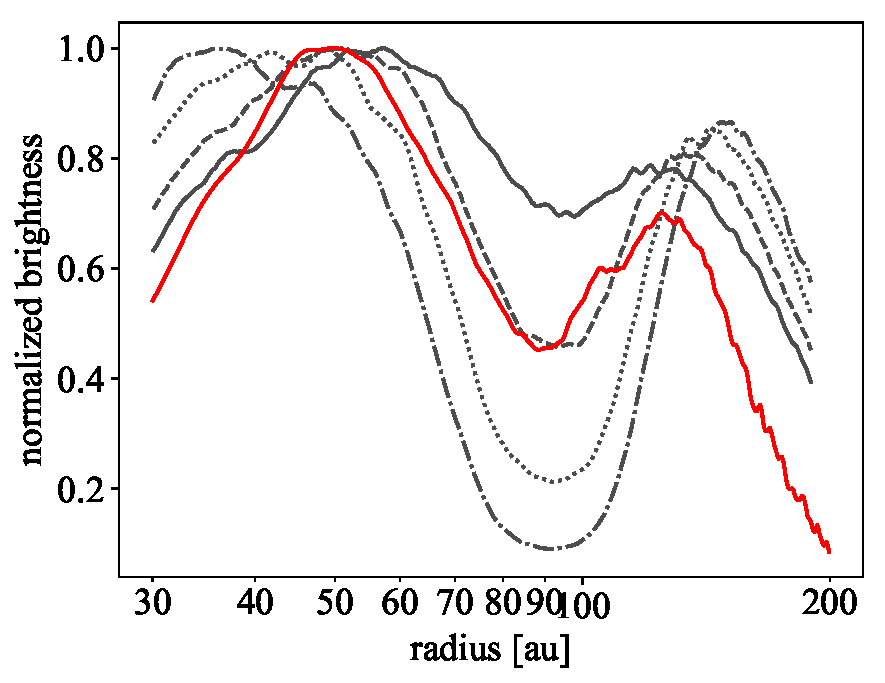
\includegraphics[width=1.00\columnwidth]{figs/scattered-radial.pdf}
      \caption{Azimuthally-averaged radial profile of $1.6$~$\mu$m polarized
         intensity scaled by $R^2$. The solid, dashed, dotted, and dot-dashed
         lines are for 0.1, 0.3, 1, and 2~$\mathrm{M_J}$ gas-only models after
         45 orbits. The red line is H-band SPHERE data from
         \citet{van-boekel:2017}.  Each line is normalized to the bright ring
         peak at $\approx$~40--50~au.\label{fig:scattered-radial}}
   \end{center}
\end{figure}










\section{Summary}
\label{sec:summary}

We have performed global three-dimensional SPH simulations of a dusty disc with
embedded protoplanets and produced synthetic observations of dust continuum, CO
emission, and polarized scattered light to test our model against recent
observations.

\begin{enumerate}
   \item We reproduce the gaps in dust emission in the ALMA observations of
      TW~Hya with a 16--24~$\earth{}$ planet at 24~au and an 8--16~$\earth{}$
      planet at 41~au, respectively.
   \item We show that a giant planet (0.1--2.0~$\mathrm{M_J}$) at 94~au can
      explain the main gap in scattered light observations, and is consistent
      with CO observations. However, a spiral arm is also evident, for which
      there is only tentative evidence in the SPHERE image.
   \item Our model requires a disc mass $\lesssim10^{-3}\,\sun{}$ in agreement
      with CO observations rather than the $>0.05\,\sun{}$ disc mass inferred
      by \citet{bergin:2013}. A low mass disc is consistent with recent
      constraints on disc turbulence \citep{flaherty:2018}.
\end{enumerate}










\section*{Acknowledgements}

DM is funded by a Research Training Program Stipend from the Australian
government. We acknowledge Australia Research Council funding via DP180104235,
FT130100034, and FT170100040. We used gSTAR and OzStar, funded by Swinburne
University of Technology and the Australian government, the MonARCH cluster at
Monash, and \textsc{splash} \citep{price:2007}.


\bibliography{references}
\label{lastpage}

\end{document}
